\chapter{Analysis}

\section{Introduction}

\subsection{Client Identification}
My client is Ian Vines. He works for the company Huxley Bertram which is an engineering company that focuses on designing and making machines for other companies. \par

My client is involved in the design of the machines. This process involves drawing the required machine using a computer program including all the parts needed in the design. When the design has been verified and given over to the engineers who build the machine, the parts required are checked and any that are low in stock are ordered from suppliers. Specific parts are ordered from different suppliers so not all of the parts are ordered from the same company. The parts are then ordered and delivered to Huxley Bertram.
\subsection{Define the current system}
The current system is a spreadsheet containing all of the suppliers information. Currently the system does not provide which company provides which part and one of the managers has to be asked which company to go to. The spreadsheet is not organised in any form and all of the supplier's information is recorded in an unstructured format. Changes to any of the information has to be done by manually finding the information to edit and deleting the incorrect information and replacing it with the appropriate information
\subsection{Describe the problems}
The company currently gets machine parts from all different companies and people and at the moment the only information they have about the companies is on the text document. To find out what company they get a certain machine part from they have to go through all the pages to find the right one. This takes a lot of time and they need a system that can make the process a lot quicker.

\section{Investigation}

\subsection{The current system}
A text document/Notepad/spreadsheet with the information that is needed to buy the part from the company. It usually consists of the company's name, address, email, phone number, postcode, website name, part name and part price. To edit the document it needs to be done manually by finding what you want to change and then manually editing it by deleting the incorrect information and retyping the correct information. There is currently no organisation within the document.

\textbf{Client interview(typed up) on following pages}\\

\begin{center}
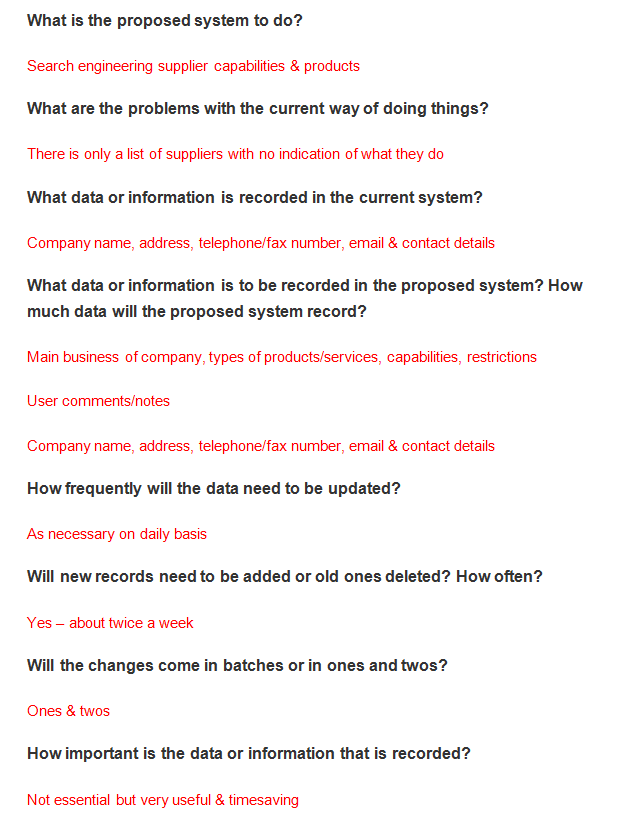
\includegraphics{InterviewPart1.jpg}
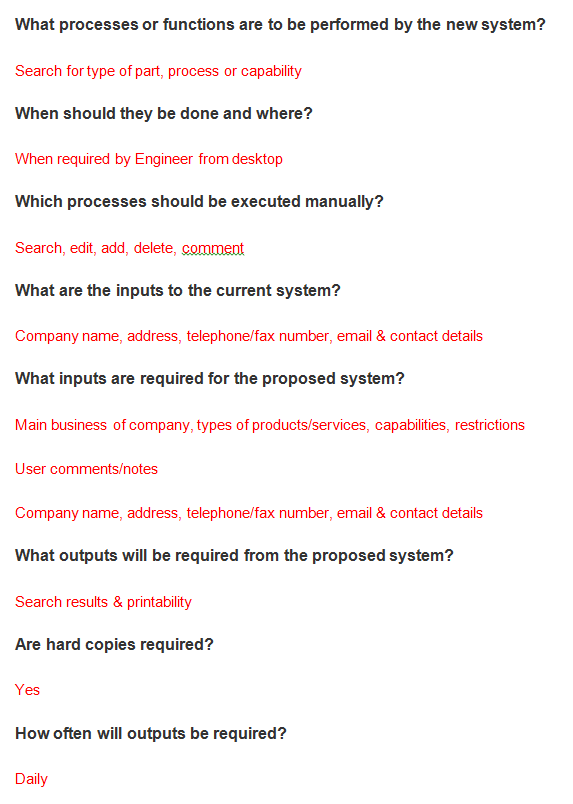
\includegraphics{InterviewPart2.jpg}
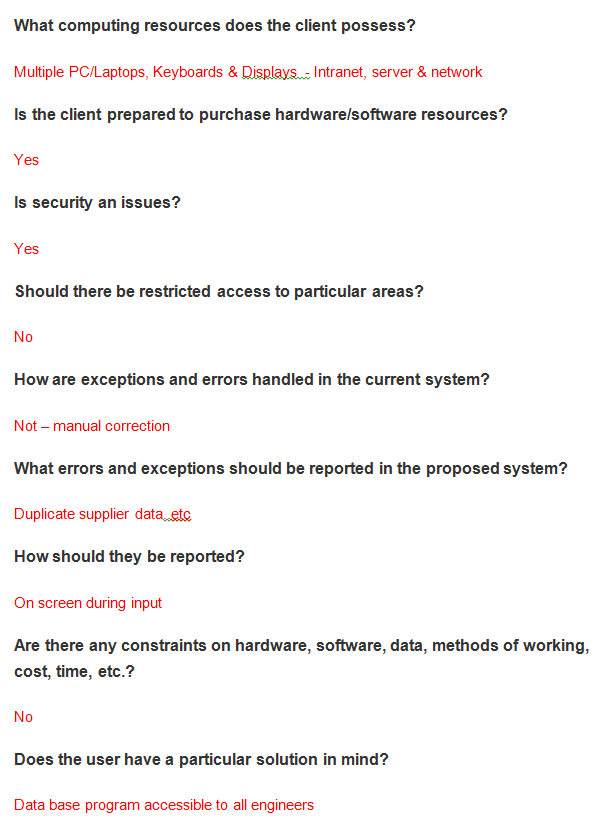
\includegraphics{InterviewPart3.jpg}
\end{center}



\subsubsection{Data sources and destinations}

\begin{center}
\begin{tabular}{ |c|c|c| } 
\hline
\bf\underline{Data}                                                                                                      & \bf\underline{Data Source} & \bf\underline{Data Destination}

\\
\hline
\ Company Name & Fax/Email & Spreadsheet\\
\hline
\ Company Address & Fax/Email & Spreadsheet\\ 
\hline
\ Company Telephone Number & Fax/Email & Spreadsheet\\
\hline
\ Company's Owner Name & Fax/Email & Spreadsheet\\
\hline
\ Company's Website & Fax/Email/Online & Spreadsheet\\
\hline
\ Part Required Information & Company Website/Email & Spreadsheet\\
\hline
\ Part Required Price & Company Website/Email & Spreadsheet\\
\hline
\end{tabular}
\end{center}
\subsubsection{Algorithms}

search document\\\
if part name is part looking for\\
get company information\\
else\\
keep looking

\subsubsection{Data flow diagram}
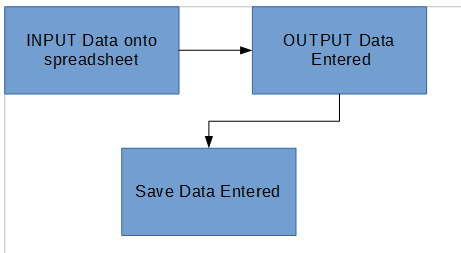
\includegraphics{FCCS.jpg}
\clearpage

\subsection{The proposed system}
The proposed system will be a database that stores all of the different company's information and which machine part they are selling. The program will allow you to add or remove companies from the database according to any new information you receive. It will also allow you to edit the information stored in the data base allowing you to update any changes that may have happened. You will also be allowed to search key words such as a company's name or the specific part you need. The program will then show all the appropriate companies with the part you need,the price and the company's contact information. The program will also show the comments of other employees on what they thought of the product and if it suited their needs.

\subsubsection{Data sources and destinations}
\begin{center}
\begin{tabular}{ |c|c|c| } 
\hline
\bf\underline{Data}                                                                                                      & \bf\underline{Data Source} & \bf\underline{Data Destination}

\\
\hline
\ Company Name & Fax/Email & Database\\
\hline
\ Company Address & Fax/Email & Database\\ 
\hline
\ Company Telephone Number & Fax/Email & Database\\
\hline
\ Company's Owner Name & Fax/Email & Database\\
\hline
\ Company's Website & Fax/Email/Online & Database\\
\hline
\ Part Required Information & Company Website/Email & Database\\
\hline
\ Part Required Price & Company Website/Email & Database\\
\hline
\end{tabular}
\end{center}
\subsubsection{Algorithms}

\underline{Search for part}\\
if part is same as part searched for\\
output company information\\
elif\\
if part is not the same as part searched for\\
do not display\\
else\\
part is not valid

\underline{Adding a part}\\
while confirm is no\\
output please enter a part and the corresponding company information\\
input part and information\\
output confirm\\
if confirm is yes\\
add to database\\
else \\
confirm is no

\underline{Deleting a part}\\
while confirm is no\\
output please enter a part to remove\\
input part\\
output confirm\\
if confirm is yes\\
delete from database\\
else \\
confirm is no

\subsubsection{Data flow diagram}
\begin{flushleft}
\textbf{Search Function}\\
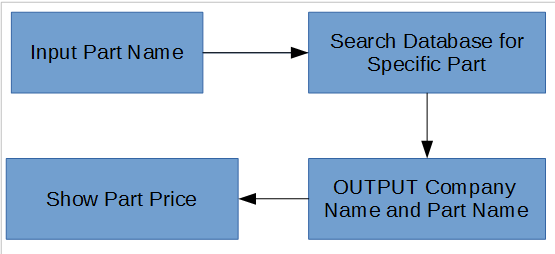
\includegraphics[scale=0.7]{FC1.jpg}\\
\clearpage
\textbf{Edit Function}\\\par
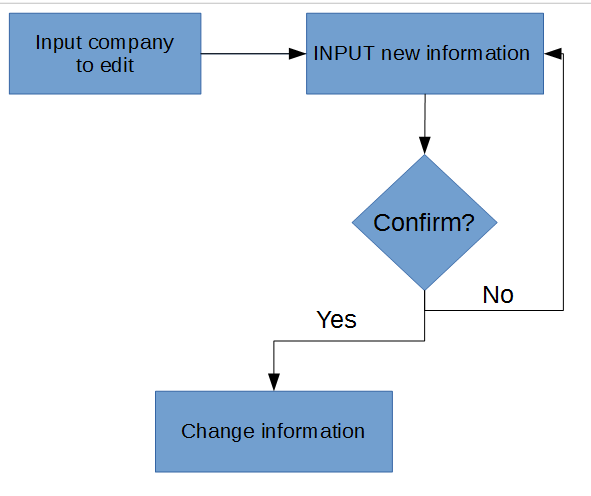
\includegraphics[scale=0.71]{FC2.jpg}\\
\textbf{Delete Function}\\
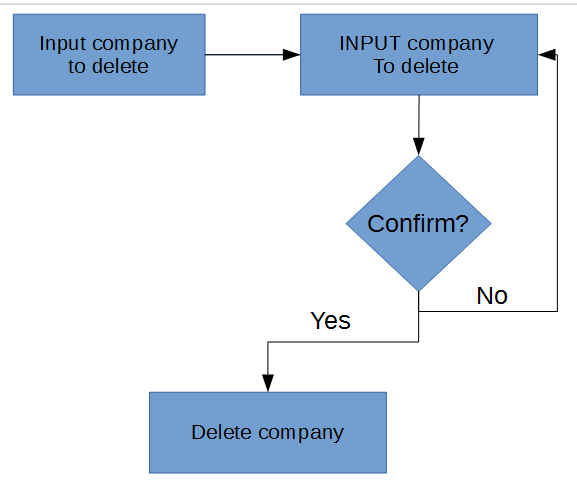
\includegraphics[scale=0.7]{FC3.jpg}\\
\textbf{Add Function}\\\par
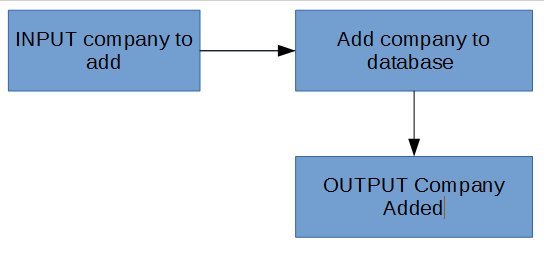
\includegraphics[scale=0.7]{FC4.jpg}\\
\end{flushleft}
\clearpage

\subsubsection{Data dictionary}
\begin{center}
\begin{tabular}{ | m{3cm} | m{2cm} | m{2cm} | m{3cm} | m{3cm} | } 
\hline
\underline{\bf Name}& \bf\underline{Data Type} & \bf\underline{Length} & \bf\underline{Validation} & \bf\underline{Example}

\\
\hline
\ Company Name & String & Unlimited & Make sure the data is a string and not any other data type & The Name Company\\ 
\hline
\ Company Address & String and Integer & 0 to 26 characters & Maximum of 26 characters, Information is actually there and it is a string with integers & Example Address\\
\hline
\ Company Phone Number & Integer & 11 integers & Make sure the input is not blank and is correct data type & 01234 567890\\
\hline
\ Company Email & String & Unlimited characters & No blank input. Data is correct data type & 123@example.com\\
\hline
\ Company Website & String & Unlimited characters & No blank input. Data is correct data type & www.example.com\\
\hline
\ Part Price & float & Unlimited characters & No blank input. Data is correct data type & £9.99\\
\hline
\ Part Name & String & Unlimited characters & No blank input. Data is correct data type & Screw\\
\hline
\end{tabular}
\end{center}
\subsubsection{Volumetrics}
The system should be able to store at least 200 supplier's information along with the part they provide and the price. It should allow for expansion to allow more information to be stored. 

\section{Objectives}

\subsection{General Objectives}
\begin{itemize}
	\item Menu must be easy to use and interact with
	\item The search must function quickly and must be easy to use
	\item The information stored must be easy to retrieve and access
	\item The company shown must be relevant to the part required
\end{itemize}

\subsection{Specific Objectives}
\begin{itemize}
	\item The user is able to edit the information 
	\item The price of the part is shown
	\item The Rating of the part is shown
	\item Employees can add comments about certain parts and companies
	\item Database can hold over 20 attributes
	\item The user is able to add/delete information
\end{itemize}
\subsection{Core Objectives}
\begin{itemize}
	\item The user is able to edit the information 
	\item The price of the part is shown
	\item The Rating of the part is shown
	\item Employees can add comments about certain parts and companies
\end{itemize}
\subsection{Other Objectives}
\begin{itemize}
	\item able to print information
	\item able to delete information
\end{itemize}
\section{ER Diagrams and Descriptions}

\subsection{ER Diagram}
\begin{center}
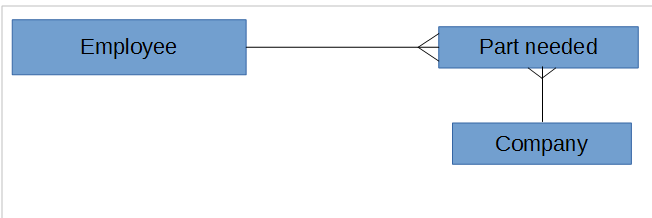
\includegraphics[width =\textwidth]{ERDiagram.jpg}
\end{center}

\subsection{Entity Descriptions}
\textbf{Employee}(First Name, Last Name, ID) \\
\textbf{Part Needed}(Part Name, Part Size, Part Price) \\
\textbf{Company Information}(Company Name, Email Address, Telephone Number, Website, Company Owner)  \\
\section{Object Analysis}

\subsection{Object Listing}
\begin{itemize}
	\item Employee
	\item Part Needed
	\item Company information
\end{itemize}

\subsection{Relationship diagrams}

\subsection{Class definitions}
\begin{center}
\begin{tabular}{ |c| }
\hline
\textbf{Employee}\\
\hline
FirstName\\
LastName\\
ID\\
\hline
GetUserFirstName\\
GetUserLastName\\
GetUserID\\
\hline
\end{tabular}
\end{center}
\begin{center}
\begin{tabular}{ |c| }
\hline
\textbf{PartNeeded}\\
\hline
PartName\\
PartSize\\
PartPrice\\
\hline
GetPartName\\
GetPartSize\\
ShowPartName\\
ShowPartSize\\
ShowPartPrice\\
\hline
\end{tabular}
\end{center}
\begin{center}
\begin{tabular}{ |c| }
\hline
\textbf{CompanyInformation}\\
\hline
Attribute\\
CompanyName\\
CompanyEmail\\
CompanyNumber\\
CompanyWebsite\\
CompanyOwner\\
\hline
AddCompany\\
DeleteCompany\\
EditCompany\\
GetCompanyName\\
ShowCompanyName\\
DeleteCompanyName\\
EditCompanyName\\
GetCompanyEmail\\
ShowCompanyEmail\\
DeleteCompaEmail\\
EditCompanyEmail\\
GetCompanyNumber\\
ShowCompanyNumber\\
DeleteCompanyNumber\\
EditCompanyNumber\\
GetCompanyWebsite\\
ShowCompanyWebsite\\
DeleteCompanyWebsite\\
EditCompanyWebsite\\
GetCompanyOwner\\
ShowCompanyOwner\\
DeleteCompanyOwner\\
EditCompanyOwner\\
\hline
\end{tabular}
\end{center}
\begin{center}
\begin{tabular}{ |c| }
\hline
\textbf{CommentsSection}\\
\hline
Comment\\
\hline
AddComment\\
DeleteComment\\
ShowComment\\
\hline
\end{tabular}
\end{center}
\begin{center}
\begin{tabular}{ |c| }
\hline
\textbf{PrintFunctionality}\\
\hline
Print\\
\hline
PrintInformation\\
PrintAll\\
\hline
\end{tabular}
\end{center}

\section{Constraints}

\subsection{Hardware}
The hardware available is the basic computer hardware. This includes: A mouse, A keyboard, A monitor, A computer, Speakers. Anything else must be discussed with the client to see if the company is willing to buy the additional hardware.

\subsection{Software}
The software available must be downloadable (if needed) and must be available to Windows 7,8 and 10. It should be easily accessed to every user and should run on most if not all computers.
\subsection{Time}
The deadline for the project is april 2015.
\subsection{User Knowledge}
The system must be simple and easy to use by someone who is not familiar with all the functions on a computer. It must have a layout that is easy to access the information and has everything that is needed within one window. There shouldn't be multiple windows open.
\subsection{Access restrictions}
Every employee should be allowed to use the software so there are no access restrictions.

\section{Limitations}

\subsection{Areas considered for future computerisation}
Making the database online so that it is easier to use in multiple locations such as at home. This also allows it to be updated in realtime.
\section{Solutions}

\subsection{Alternative solutions}
\textbf{\underline{Spreadsheet}}
\\
\\
{Advantages}
\begin{itemize}
	\item Can hold all of the information about each company and each part
	\item Can be stored as a table
	\item Can add/remove data
\end{itemize}
{Disadvantages}
\begin{itemize}
	\item Can't search for a specific part
	\item Not easy to find information
	\item Will not prioritize parts according to review left by other employees
	\item May need specific program downloaded
	\item It is what the current system is already which is not 
\end{itemize}
\textbf{\underline{Database}}
\\
\\
{Advantages}
\begin{itemize}
	\item Can hold all of the information about each company and each part
	\item Can be searched for specific items
	\item Can filter searches to user specifications 
	\item Can add/remove data
	\item Can hold a wide range of data
\end{itemize}
{Disadvantages}
\begin{itemize}
	\item May need specific program downloaded
	\item Limited to interface
	\item Limited to features included
\end{itemize}
\textbf{\underline{Writing a Program}}
\\
\\
{Advantages}
\begin{itemize}
	\item Can Include a database if needed
	\item Can Customize to include a whole range of features
	\item Can Filter searches to user specifications 
	\item Can Add/remove data
	\item Can Create a simple and easy to use interface
\end{itemize}
{Disadvantages}
\begin{itemize}
	\item May need specific program downloaded
	\item Can take time to write
	\item Can contain lots of errors if done incorrectly
\end{itemize}
\subsection{Justification of chosen solution}
The chosen solution will be writing a program as it allows for the biggest range of customization  to suit to the users needs. Although a program can contain a lot of errors if done incorrectly, the errors can be easy to fix. The only problem with writing a program is that it could take more time then perhaps other alternative, but the overall quality of the program compared to the other options in the end will be better suited to the client. The program will also include a database to store the information as i feel that it is the best way to store the information as spreadsheets  can be hard to read if you have a load of data to use. Also a spreadsheet is what the current system is and the client wants something different to this.